\section{Cache}
\label{sec:cache}
\sources{Lecture ``Memory Hierarchy Design'' (\nolinkurl{04-cache-lecture.pdf});
Group~1 ``Cache'' (\nolinkurl{04-cache-group1.pdf}); H\&P 5th ed.\ App.~B
(\S B.1--B.3) and Ch.~2 (\S2.1--2.2).}

% =============================================================================
\subsection{The Memory Hierarchy}
\label{sec:hierarchy}

\paragraph{The processor--memory gap.} Since 1980 processor performance has
grown about 60\% per year but DRAM latency only about 9\% per year, so the gap
grew about 50\% per year. A four-issue 2~GHz superscalar waiting on a 100~ns DRAM
access could have executed 800 instructions in that time. The goal of the
hierarchy is the \emph{illusion of a memory as large as the cheapest level and as
fast as the fastest}.\HP{\S2.1, Figure~2.2}{74}

\begin{center}
\small
\begin{tabular}{@{}lllll@{}}
\toprule
Level & Typical size & Technology & Access time & Managed by \\
\midrule
Registers & $<1$ KB & custom CMOS & 0.15--0.3 ns & compiler \\
Cache & 32 KB--8 MB & on-chip SRAM & 0.5--15 ns & hardware \\
Main memory & $<512$ GB & DRAM & 30--200 ns & operating system \\
Disk & $>1$ TB & magnetic disk / flash & $\approx5{,}000{,}000$ ns & OS / operator \\
\bottomrule
\end{tabular}
\end{center}
Moving down the hierarchy, each level is larger, slower and cheaper per byte; the
unit moved between levels grows: words (registers), \textbf{blocks} or lines of
8--128 bytes (cache), \textbf{pages} of 4--64 KB (memory).\HPA{B}{\S B.1, Figure~B.1}{3}

\begin{definition}[Locality]
\textbf{Temporal locality}: a location referenced now is likely to be referenced
again soon (loops, reused variables). \textbf{Spatial locality}: locations near
one just referenced are likely to be referenced soon (sequential code, array
traversal). Rule of thumb: a program spends 90\% of its time in 10\% of its
code. Caches exploit temporal locality by \emph{keeping} recently used data and
spatial locality by fetching whole \emph{blocks}.
\end{definition}

\begin{definition}[Basic terms]
A \textbf{block} (line) is the unit copied between two adjacent levels. A
\textbf{hit}: the data is found in the upper level; \textbf{hit time} is the time
to access it, including deciding hit or miss. A \textbf{miss}: the block must be
fetched from the lower level; the \textbf{miss penalty} is the time to replace a
block and deliver the data to the processor. Hit rate $=$ hits/accesses; miss rate
$=1-$ hit rate.\HPA{B}{\S B.1}{2}
\end{definition}

\begin{eg}[Locality in a loop]
\texttt{for (i = 0; i < 10; i++) S = S + A[i];} Without a cache this makes at
least 12 memory accesses (10 reads of \texttt{A[i]}, read and write \texttt{S}). If
\texttt{A[0..9]} and \texttt{S} fit in one 32-byte block, the cache needs one
access to load the block and one to write it back. \texttt{S} shows temporal
locality, \texttt{A[i]} spatial locality.
\end{eg}

% =============================================================================
\subsection{The Four Questions}
\label{sec:four-questions}

Every level of the hierarchy answers four questions:\HPA{B}{\S B.1}{6}
\begin{enumerate}
  \item \textbf{Block placement}: where can a block be placed? (direct mapped,
  set associative, fully associative)
  \item \textbf{Block identification}: how is a block found? (tag, index, valid bit)
  \item \textbf{Block replacement}: which block is replaced on a miss? (random,
  LRU, FIFO and LRU approximations)
  \item \textbf{Write strategy}: what happens on a write? (write-through or
  write-back; write allocate or not)
\end{enumerate}

\subsubsection{Q1: Block placement}
\begin{definition}[Cache organizations]
With $C$ = cache size, $B$ = block size and $a$ = associativity:
\begin{itemize}
  \item \textbf{Direct mapped}: each block has exactly one place,
  (block address) mod (number of blocks).
  \item \textbf{$n$-way set associative}: the cache has $S=C/(B\cdot n)$
  \emph{sets} of $n$ blocks (\emph{ways}); a block goes in set
  (block address) mod $S$, in any of its ways.
  \item \textbf{Fully associative}: a block can go anywhere (one set).
\end{itemize}
Direct mapped is 1-way set associative; fully associative with $m$ blocks is
$m$-way set associative.\HPA{B}{\S B.1, Figure~B.2}{7}
\end{definition}

\begin{center}\begin{minipage}{\linewidth}\centering
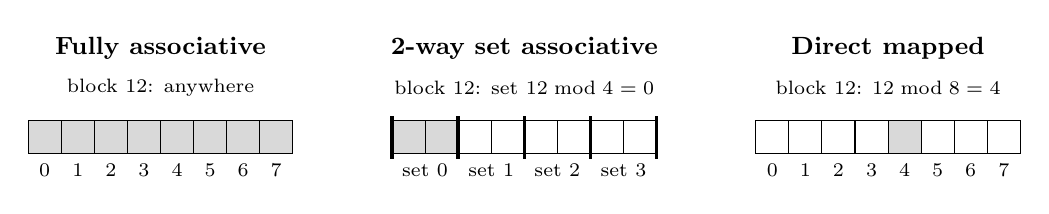
\begin{tikzpicture}[font=\scriptsize,x=0.42cm,y=0.42cm]
  \node[font=\small\bfseries] at (4,3.2) {Fully associative};
  \fill[black!15] (0,0) rectangle (8,1);
  \foreach \i in {0,...,7} {\draw (\i,0) rectangle ++(1,1); \node at (\i+0.5,-0.5) {\i};}
  \node at (4,2) {block 12: anywhere};
  \node[font=\small\bfseries] at (15,3.2) {2-way set associative};
  \fill[black!15] (11,0) rectangle (13,1);
  \foreach \i in {11,...,18} {\draw (\i,0) rectangle ++(1,1);}
  \foreach \x in {11,13,15,17,19} {\draw[very thick] (\x,-0.15) -- (\x,1.15);}
  \foreach \s/\x in {0/12,1/14,2/16,3/18} {\node at (\x,-0.5) {set \s};}
  \node at (15,2) {block 12: set $12 \bmod 4 = 0$};
  \node[font=\small\bfseries] at (26,3.2) {Direct mapped};
  \fill[black!15] (26,0) rectangle (27,1);
  \foreach \i/\n in {22/0,23/1,24/2,25/3,26/4,27/5,28/6,29/7} {\draw (\i,0) rectangle ++(1,1); \node at (\i+0.5,-0.5) {\n};}
  \node at (26,2) {block 12: $12 \bmod 8 = 4$};
\end{tikzpicture}
\diagramsource{\nolinkurl{04-cache-lecture.pdf}, handout p.~4, slide 14 (``Q1: Where can a block be placed?''); Group~1 slide 19 (``Q1: Where Can a Block Be Placed in a Cache?''); cf.\ H\&P Fig.~B.2, \hppage{B}{8}}
\end{minipage}
\end{center}
\noindent An 8-block cache and memory block 12: the shaded frames are where it may
go.

\begin{itemize}
  \item \textbf{Direct mapped}: simple and fast, but a high miss rate when two
  busy blocks share an index (the ``ping-pong'' effect): a block is replaced while
  other frames are empty.
  \item \textbf{Fully associative}: needs a comparator per block (content
  addressable memory, CAM); a block is replaced only when the cache is full; costly
  in area, power and delay, so used only for small structures (TLBs).
  \item \textbf{Set associative}: the compromise used in practice (Intel, AMD:
  2- to 16-way); $n$ comparators and an $n$-to-1 multiplexer.
\end{itemize}

\subsubsection{Q2: Block identification}
\begin{center}\begin{minipage}{\linewidth}\centering
\begin{tikzpicture}[font=\small]
  \node[draw,minimum width=4.6cm,minimum height=0.6cm] (t) {Tag};
  \node[draw,minimum width=3cm,minimum height=0.6cm,right=0pt of t] (i) {Index};
  \node[draw,minimum width=2.4cm,minimum height=0.6cm,right=0pt of i] (o) {Block offset};
  \node[font=\scriptsize,below=1pt of t] {$t=A-k-b$ bits};
  \node[font=\scriptsize,below=1pt of i] {$k=\log_2 S$ bits};
  \node[font=\scriptsize,below=1pt of o] {$b=\log_2 B$ bits};
  \draw[decorate,decoration={brace,amplitude=4pt}] (t.north west) -- node[above=4pt,font=\scriptsize]{block address $=\lfloor\text{addr}/B\rfloor$} (i.north east);
\end{tikzpicture}
\diagramsource{\nolinkurl{04-cache-lecture.pdf}, handout p.~7, slide 25 (``Q2: How is a block found?''); Group~1 slide 31; cf.\ H\&P Fig.~B.3, \hppage{B}{9}}
\end{minipage}
\end{center}
\begin{prop}[Address fields]
For an $A$-bit byte address: \textbf{offset} $b=\log_2 B$ bits selects the byte in
the block; \textbf{index} $k=\log_2 S$ bits selects the set; the remaining
$t=A-k-b$ bits are the \textbf{tag}, compared with the tags stored in every way of
the set. A \textbf{valid bit} per block says whether the entry holds data (it is 0
after reset).\HPA{B}{\S B.1, Figure~B.3}{8}
\[
  S=\frac{C}{B\times a},\qquad \text{set}=\text{block address}\bmod S,\qquad
  \text{tag}=\left\lfloor\frac{\text{block address}}{S}\right\rfloor .
\]
\end{prop}
\begin{itemize}
  \item With $C$ and $B$ fixed, doubling the associativity halves the sets: the
  index loses a bit and the tag gains one. Fully associative caches have no index.
  \item Storage per block $=8B$ data bits $+$ tag $+$ valid ($+$ dirty for
  write-back) ($+$ replacement state).
\end{itemize}

\begin{eg}[Three caches from the slides]
All with 32-bit byte addresses.
\begin{center}
\small
\begin{tabular}{@{}lllll@{}}
\toprule
Cache & Blocks & Offset & Index & Tag \\
\midrule
4 KB direct mapped, 1-word blocks & 1024 & 2 & 10 & 20 \\
64 KB direct mapped, 4-word blocks & 4096 & 4 & 12 & 16 \\
4 KB 4-way, 1-word blocks (256 sets) & 1024 & 2 & 8 & 22 \\
\bottomrule
\end{tabular}
\end{center}
The 64 KB cache uses the 2 offset bits above the byte offset to select one of the
4 words (a multiplexer). The 4-way cache compares 4 tags in parallel and selects
the hit way with a 4-to-1 multiplexer, which lengthens the hit time.
\end{eg}

\begin{eg}[Mapping a byte address]
A direct-mapped cache has 64 blocks of 16 bytes. Byte address 1200 is in memory
block $\lfloor1200/16\rfloor=75$ (bytes 1200--1215), which maps to cache block
$75\bmod64=11$. In bits: offset $=$ low 4 bits, index $=$ next 6 bits $=001011_2=11$.
\end{eg}

\subsubsection{Q3: Block replacement}
Direct mapped has no choice. For set-associative and fully associative caches:
\begin{itemize}
  \item \textbf{Random}: spread allocation uniformly; often pseudo-random so
  behaviour is reproducible for debugging. Simplest hardware.
  \item \textbf{Least recently used (LRU)}: replace the block unused for the
  longest time (a corollary of locality). The state must be updated on every
  access; exact LRU needs the full order of the $n$ ways ($\lceil\log_2 n!\rceil$
  bits per set), so it is only feasible for small sets (2- or 4-way).
  \item \textbf{First in, first out (FIFO)}, also round-robin: replace the oldest
  block; hits do not change the order. Used in highly associative caches.
\end{itemize}
Replacement has a \emph{second-order} effect: it acts only on misses. For large
caches LRU, random and FIFO differ by under 1\%; for a 16~KB 2-way cache the
data misses per 1000 instructions are 114.1 (LRU), 117.3 (random), 115.5
(FIFO).\HPA{B}{\S B.1, Figure~B.4}{10}

\paragraph{LRU approximations.}
\begin{itemize}
  \item \textbf{Tree pseudo-LRU} (the lecturer's slides; common for 4--8 ways):
  $n-1$ bits form a binary tree over the ways. For 4 ways, $b_0$ chooses the pair
  ($\{0,1\}$ or $\{2,3\}$), $b_1$ the way in $\{0,1\}$, $b_2$ the way in $\{2,3\}$.
  On every access the bits on the path are set to point \emph{away} from the
  accessed way; the victim is found by following the bits from the root.
  \item \textbf{One bit per way} (the pseudo-LRU of H\&P): an access sets the bit
  of its way; when all bits of a set are 1 they are cleared except the newest; the
  victim is a way whose bit is 0.\HPA[10]{B}{\S B.1}{9}
  \item \textbf{Clock} (second chance): the ways form a circle with one reference
  bit each and a pointer. An access sets the bit. To replace, look at the pointed
  way: if its bit is 1, clear it and advance; replace the first way whose bit is 0.
  The new block gets bit 1 and the pointer moves past it. The same algorithm
  approximates LRU for pages (Section~\ref{sec:vm-replacement}).
\end{itemize}

\begin{center}\begin{minipage}{\linewidth}\centering
\begin{tikzpicture}[font=\small,level distance=1.1cm,
  level 1/.style={sibling distance=3.6cm},level 2/.style={sibling distance=1.6cm}]
  \node[tnode] {$b_0$}
    child {node[tnode] {$b_1$}
      child {node[box] {way 0} edge from parent node[left,font=\scriptsize]{0}}
      child {node[box] {way 1} edge from parent node[right,font=\scriptsize]{1}}
      edge from parent node[left,font=\scriptsize]{0}}
    child {node[tnode] {$b_2$}
      child {node[box] {way 2} edge from parent node[left,font=\scriptsize]{0}}
      child {node[box] {way 3} edge from parent node[right,font=\scriptsize]{1}}
      edge from parent node[right,font=\scriptsize]{1}};
  \node[align=left,font=\scriptsize,anchor=west] at (4.2,-1.2)
    {Access way 0: $b_0\leftarrow1$, $b_1\leftarrow1$\\
     Access way 2: $b_0\leftarrow0$, $b_2\leftarrow1$\\
     Victim: follow $b_0$, then $b_1$ or $b_2$};
\end{tikzpicture}
\diagramsource{own diagram; the lecturer's slide 28 (\nolinkurl{04-cache-lecture.pdf}, handout p.~8) only names ``pseudo-LRU binary tree''; bit convention as defined in the text, traced in the example below}
\end{minipage}
\end{center}

\begin{eg}[Four policies on one 4-way set]
Block references \texttt{0 1 2 3 0 4 1 0 5 2 3 0}, set initially empty (fill ways
0--3 in order; tree bits $b_0b_1b_2$ start at 000; Clock gives new blocks bit 1).
M $=$ miss (victim), H $=$ hit.
\begin{center}
\scriptsize
\setlength{\tabcolsep}{2.4pt}
\begin{tabular}{@{}lcccccccccccc@{}}
\toprule
Ref & 0 & 1 & 2 & 3 & 0 & 4 & 1 & 0 & 5 & 2 & 3 & 0 \\
\midrule
LRU & M & M & M & M & H & M(1) & M(2) & H & M(3) & M(4) & M(1) & H \\
FIFO & M & M & M & M & H & M(0) & H & M(1) & M(2) & M(3) & M(4) & H \\
Tree & M & M & M & M & H & M(2) & H & H & M(3) & M(1) & M(4) & H \\
\quad $b_0b_1b_2$ & 110 & 100 & 001 & 000 & 110 & 011 & 101 & 111 & 010 & 100 & 001 & 111 \\
Clock & M & M & M & M & H & M(0) & H & M(2) & M(3) & M(1) & M(4) & H \\
\bottomrule
\end{tabular}
\end{center}
Misses: LRU 9, FIFO 9, Tree 8, Clock 9. At reference 4 the tree bits are 110
($b_0=1$: right pair; $b_2=0$: way 2), so the tree evicts block 2 while true LRU
evicts block 1: tree PLRU only approximates LRU (here, by luck, it does better).
Clock at reference 4 finds every bit set, clears all four and evicts block 0.
\end{eg}

\subsubsection{Q4: Write strategy}
Reads dominate: with 26\% loads and 10\% stores, writes are about 7\% of all
memory traffic and 28\% of data-cache traffic. A read can access the block while
the tag is checked; a write cannot modify the block until the tag matches, so
writes are slower.\HPA[11]{B}{\S B.1}{10}
\begin{definition}[Write policies]
On a write \textbf{hit}:
\begin{itemize}
  \item \textbf{Write-through}: write both the cache block and the lower level.
  Simple; the lower level always has the current data (simplifies coherence and
  I/O); a read miss never causes a write. Uses a \textbf{write buffer} so the
  processor need not wait (\emph{write stall} otherwise).
  \item \textbf{Write-back}: write only the cache; a modified block is written to
  the lower level when it is replaced. A \textbf{dirty bit} marks modified blocks so
  clean blocks are not written back. Writes run at cache speed, several writes to
  a block cost one write-back, less bandwidth and power.
\end{itemize}
On a write \textbf{miss}:
\begin{itemize}
  \item \textbf{Write allocate} (fetch on write): load the block, then write as on
  a hit.
  \item \textbf{No-write allocate}: write only the lower level; the cache is not
  changed.
\end{itemize}
Usual pairs: write-back $+$ write allocate; write-through $+$ no-write
allocate.\HPA[12]{B}{\S B.1}{11}
\end{definition}

\begin{eg}[Write allocate vs.\ no-write allocate]
A fully associative write-back cache, initially empty, sees
\texttt{Write M[100]; Write M[100]; Read M[200]; Write M[200]; Write M[100]}.
No-write allocate: 100 is never brought in, so both writes to 100 and the last
one miss; the read of 200 misses and loads it; the write to 200 hits: \textbf{4
misses, 1 hit}. Write allocate: only the first accesses to 100 and 200 miss:
\textbf{2 misses, 3 hits}.\HPA{B}{\S B.1, Example}{12}
\end{eg}

\begin{eg}[A real cache: AMD Opteron L1 data cache]
64 KB, 64-byte blocks, 2-way set associative, LRU, write-back, write allocate. So
$64\text{K}/(64\times2)=512$ sets: 9 index bits, 6 offset bits; the 40-bit
physical address leaves a $40-9-6=25$-bit tag. A victim buffer holds blocks being
written back.\HPA[14]{B}{\S B.1, Figure~B.5}{12}
\end{eg}

% =============================================================================
\subsection{Cache Performance}
\label{sec:cache-perf}

\begin{theorem}[CPU time with memory stalls]
\begin{align*}
  \text{CPU time} &= (\text{CPU clock cycles}+\text{Memory stall cycles})\times\text{Clock cycle time}\\
  \text{Memory stall cycles} &= \text{IC}\times\frac{\text{Misses}}{\text{Instruction}}\times\text{Miss penalty}\\
  &= \text{IC}\times\frac{\text{Memory accesses}}{\text{Instruction}}\times\text{Miss rate}\times\text{Miss penalty}
\end{align*}
Every instruction makes one instruction fetch, plus a data access if it is a
load or store. Hit cycles are counted in the CPU clock cycles.\HPA[5]{B}{\S B.1}{4}
\end{theorem}

\begin{eg}[Cost of misses]
$\CPI=1.0$ when all accesses hit; loads and stores are 50\% of instructions; miss
penalty 25 cycles; miss rate 2\%. Stall cycles per instruction
$=(1+0.5)\times0.02\times25=0.75$, so $\CPI=1.75$: the perfect cache would be
$1.75\times$ faster.\HPA{B}{\S B.1, Example}{5}
\end{eg}

\begin{definition}[Average memory access time]
\[
  \AMAT=\text{Hit time}+\text{Miss rate}\times\text{Miss penalty}.
\]
It is a better measure than miss rate, but still not a substitute for execution
time.\HPA{B}{\S B.2}{16} Misses per instruction and miss rate are related by
$\dfrac{\text{Misses}}{\text{Instruction}}=\text{Miss rate}\times\dfrac{\text{Memory accesses}}{\text{Instruction}}$;
data are often given as misses per 1000 instructions (MPKI).
\end{definition}

\begin{eg}[Split or unified cache?]
16 KB I-cache $+$ 16 KB D-cache vs.\ a 32 KB unified cache. Misses per 1000
instructions: 3.82 (16 KB I), 40.9 (16 KB D), 43.3 (32 KB unified); 36\% of
instructions are loads/stores, so 74\% of accesses are instruction fetches
($1/1.36$). Hit 1 cycle, miss penalty 200 cycles; the single-ported unified cache
adds 1 cycle to a data access (structural hazard).
Miss rates: $3.82/1000=0.004$; $40.9/1000/0.36=0.114$;
$43.3/1000/1.36=0.0318$. Split overall $0.74(0.004)+0.26(0.114)=0.0326$.
\begin{align*}
  \AMAT_{split}&=0.74(1+0.004\cdot200)+0.26(1+0.114\cdot200)=7.52\\
  \AMAT_{unified}&=0.74(1+0.0318\cdot200)+0.26(1+1+0.0318\cdot200)=7.62
\end{align*}
The unified cache has the lower miss rate, but the split caches win on AMAT
because they give two ports per cycle.\HPA[17]{B}{\S B.2, Example and Figure~B.6}{15}
\end{eg}
\begin{remark}
\textbf{Textbook typo.} The book states a miss penalty of 100 cycles in this
example but computes with 200; the numbers above follow the book's computation.
\end{remark}

\begin{eg}[In-order processor]
Miss penalty 200 cycles, $\CPI_{exec}=1.0$, miss rate 2\%, 1.5 memory references
per instruction (30 misses per 1000 instructions):
$\CPI=1.0+1.5\times0.02\times200=1.0+30/1000\times200=7.0$. With no cache at all:
$1.0+1.5\times200=301$. The lower the $\CPI_{exec}$ and the faster the clock, the
larger the relative impact of a miss.\HPA[19]{B}{\S B.2, Example}{18}
\end{eg}

% =============================================================================
\subsection{The Three Cs}
\label{sec:three-cs}

\begin{definition}[Miss categories]
\begin{itemize}
  \item \textbf{Compulsory} (cold-start, first-reference): the very first access
  to a block. They occur even in an infinite cache.
  \item \textbf{Capacity}: the cache cannot hold all blocks the program needs, so
  blocks are discarded and later retrieved. They occur in a fully associative
  cache of the same size.
  \item \textbf{Conflict} (collision): in a set-associative or direct-mapped
  cache, too many blocks map to one set. They are the misses of an $n$-way cache
  that would hit in the fully associative cache of the same size.
\end{itemize}
Multiprocessors add a fourth C, \textbf{coherence} misses
(Section~\ref{sec:mp}).\HPA{B}{\S B.3}{23}
\end{definition}

\begin{itemize}
  \item In SPEC2000 the compulsory miss rate is tiny (0.0001); for a 4 KB cache the
  total miss rate is 0.098 direct mapped, 0.076 2-way, 0.071 4- or 8-way, and the
  capacity part alone is 0.070.\HPA{B}{\S B.3, Figure~B.8}{24}
  \item \textbf{8-way is as good as fully associative} for these sizes, and the
  \textbf{2:1 cache rule of thumb}: a direct-mapped cache of size $N$ has about the
  miss rate of a 2-way cache of size $N/2$.\HPA{B}{\S B.3}{29}
  \item The model has limits: it ignores replacement, and a miss can change
  category when the cache size changes.\HPA{B}{\S B.3}{26}
\end{itemize}

\begin{eg}[Classifying misses]
A direct-mapped cache of 4 one-word blocks (index $=$ address mod 4), initially
empty; word addresses \texttt{0 4 0 1 2 3 5 0 4 1}:
\begin{center}
\small
\begin{tabular}{@{}lcccccccccc@{}}
\toprule
Address & 0 & 4 & 0 & 1 & 2 & 3 & 5 & 0 & 4 & 1 \\
Index & 0 & 0 & 0 & 1 & 2 & 3 & 1 & 0 & 0 & 1 \\
Result & comp. & comp. & confl. & comp. & comp. & comp. & comp. & hit & cap. & cap. \\
\bottomrule
\end{tabular}
\end{center}
The third access misses only because 4 took index 0 (a 4-block fully associative
LRU cache would still hold 0): conflict. The last two also miss in the fully
associative cache (too many distinct blocks since their last use): capacity.
\end{eg}

% =============================================================================
\subsection{Six Basic Cache Optimizations}
\label{sec:basic-opt}

$\AMAT=\text{Hit time}+\text{Miss rate}\times\text{Miss penalty}$ gives three
targets.\HPA{B}{\S B.3}{22}
\begin{center}
\small
\begin{tabular}{@{}P{4.3cm}P{3.6cm}P{6cm}@{}}
\toprule
Optimization & Improves & Drawback \\
\midrule
1. Larger block size & miss rate (compulsory) & larger miss penalty; fewer blocks, so more conflict (and capacity) misses in small caches \\
2. Larger cache & miss rate (capacity) & longer hit time, cost, power \\
3. Higher associativity & miss rate (conflict) & longer hit time \\
4. Multilevel caches & miss penalty & more hardware; harder analysis \\
5. Read misses before writes & miss penalty & write buffer must be checked \\
6. Avoid address translation when indexing & hit time & needs virtually indexed caches \\
\bottomrule
\end{tabular}
\end{center}

\paragraph{1. Larger blocks.} Exploit spatial locality. The best block size
minimizes AMAT, not the miss rate: in the book's data 32 bytes is best for a 4 KB
cache and 64 bytes for larger ones. High latency and high bandwidth below favour
large blocks.\HPA[28]{B}{\S B.3, Figure~B.12}{26}

\paragraph{2--3. Larger caches, higher associativity.} The obvious cure for capacity
misses; associativity removes conflict misses, but each step can stretch the clock.
\begin{eg}[Associativity vs.\ hit time]
The clock cycle grows by $1.36\times$ (2-way), $1.44\times$ (4-way) and
$1.52\times$ (8-way) over direct mapped; hit 1 cycle, miss penalty 25 cycles. AMAT for a 4 KB direct
mapped cache: $1.00+0.098\times25=3.44$; 512 KB 8-way: $1.52+0.006\times25=1.66$.
Higher associativity pays off only up to about 8 KB; from 16 KB on, the longer
hit time outweighs the saved misses.\HPA[30]{B}{\S B.3, Example}{29}
\end{eg}

\paragraph{4. Multilevel caches.} L1 is small and fast enough to match the
processor clock; L2 is large enough to catch many accesses that would go to
memory, so it reduces the L1 miss penalty.\HPA{B}{\S B.3}{30}
\begin{theorem}[Two-level AMAT]
\[
  \AMAT=\text{Hit time}_{L1}+\text{Miss rate}_{L1}\times
  \big(\text{Hit time}_{L2}+\text{Miss rate}_{L2}\times\text{Miss penalty}_{L2}\big)
\]
\begin{itemize}
  \item \textbf{Local miss rate}: misses in a cache $/$ accesses \emph{to that
  cache} (for L2, the L1 misses). Large for L2, since L1 ``skims the cream''.
  \item \textbf{Global miss rate}: misses in a cache $/$ all memory accesses of the
  processor; for L2 it is $\text{Miss rate}_{L1}\times\text{Miss rate}_{L2}$. The
  better measure for L2.
  \item Stalls per instruction $=\dfrac{\text{Misses}_{L1}}{\text{Instr}}\times\text{Hit time}_{L2}
  +\dfrac{\text{Misses}_{L2}}{\text{Instr}}\times\text{Miss penalty}_{L2}$.
\end{itemize}
\HPA[32]{B}{\S B.3}{31}
\end{theorem}

\begin{eg}[Local and global miss rates]
1000 memory references: 40 L1 misses, 20 L2 misses; L1 hit 1 cycle, L2 hit 10
cycles, memory 200 cycles; 1.5 references per instruction. L1 miss rate $=4\%$;
L2 local $=20/40=50\%$, global $=20/1000=2\%$.
$\AMAT=1+0.04\times(10+0.5\times200)=5.4$ cycles. Per 1000 instructions there are
60 L1 and 30 L2 misses, so stalls per instruction
$=0.060\times10+0.030\times200=6.6$ cycles $=(5.4-1)\times1.5$.\HPA[32]{B}{\S B.3, Example}{31}
\end{eg}

\begin{eg}[Adding an L2 (Group 1)]
L1: hit 1 ns, miss rate 10\%, memory 100 ns. Only L1: $\AMAT=1+0.1\times100=11$ ns.
Add L2: hit 8 ns, local miss rate 20\%, penalty 105 ns:
$\AMAT=1+0.1\times(8+0.2\times105)=3.9$ ns.
\end{eg}

\begin{itemize}
  \item \textbf{Multilevel inclusion}: L1 data are always in L2 (coherence can be
  checked in L2 only). \textbf{Exclusion}: L1 data are never in L2; a miss swaps
  blocks, so a small L2 is not wasted on copies (AMD Opteron).\HPA[35]{B}{\S B.3}{34}
  \item The L1 speed affects the clock; the L2 speed affects only the L1 miss
  penalty. So L2 can be larger, more associative, with larger blocks.
\end{itemize}

\paragraph{5. Read misses before writes.} A read miss is urgent (the processor
waits); a buffered write is not. Let the read go first, but a write buffer may hold
the newest value of the address being read (a read-after-write hazard through
memory): either wait until the buffer drains or, as almost all processors do,
\textbf{check the write buffer} on a read miss. For write-back, copy a dirty victim
to a buffer, read the new block first, then write the victim.\HPA[36]{B}{\S B.3}{35}
\begin{eg}[RAW through the write buffer]
The sequence \texttt{SW R3,512(R0)}; \texttt{LW R1,1024(R0)};
\texttt{LW R2,512(R0)}, where 512 and 1024 map to the same block of a direct-mapped write-through cache. If the
write of 512 is still in the buffer when the second load misses, memory returns
the old value: $R2\ne R3$ unless the buffer is checked.
\end{eg}

\paragraph{6. Avoiding address translation.} A \emph{virtual} cache uses virtual
addresses, removing translation from the hit time, but needs protection checks and
a flush (or a process-ID tag) on a process switch, and can have aliases. The common
solution is a \textbf{virtually indexed, physically tagged} cache: index with page
offset bits while the TLB translates in parallel, then compare physical tags. This
limits $C/a\le$ page size (Section~\ref{sec:vm-cache}).\HPA[40]{B}{\S B.3}{36}

% =============================================================================
\subsection{Advanced Optimizations}
\label{sec:advanced-opt}
\beyond{} Group~1 presented the first and fifth of the ten advanced optimizations
of H\&P Ch.~2; the others are listed for completeness.\HP[96]{\S2.2, Figure~2.11}{78}
\begin{center}
\small
\begin{tabular}{@{}P{5.2cm}P{8.6cm}@{}}
\toprule
Optimization & Idea \\
\midrule
Small and simple L1 & low associativity, small size: short hit time, low power \\
Way prediction & predict the way to read next, like a direct-mapped hit time \\
Pipelined cache access & more cycles per hit but higher bandwidth (and clock) \\
Nonblocking caches & hit under miss, miss under miss: overlap misses \\
Multibanked caches & independent banks serve accesses in parallel \\
Critical word first, early restart & send the requested word before the rest of the block \\
Merging write buffer & combine writes to the same block in one buffer entry \\
Compiler optimizations & loop interchange, blocking: better locality \\
Hardware prefetching & fetch the next block(s) before they are requested \\
Compiler-controlled prefetching & prefetch instructions inserted by the compiler \\
\bottomrule
\end{tabular}
\end{center}

\begin{eg}[Small and simple L1]
Is a 32 KB 4-way L1 faster than a 32 KB 2-way one? Miss rates 3.7\% and 3.8\%;
the 4-way access time is $1.4\times$ the 2-way time; miss penalty $=15\times$ the
2-way access time. In units of the 2-way access time:
$\AMAT_{2}=1+0.038\times15=1.57$, $\AMAT_{4}=1.4+0.037\times15=1.96$. The 2-way
cache wins.\HP{\S2.2, Example}{80}
\end{eg}
\begin{remark}
\textbf{Textbook error.} The book prints $\AMAT_2=1.38$ (an arithmetic slip) and
computes $\AMAT_4=1.4+0.037\times10=1.77$, mixing the 2-way time unit (hit) with
4-way clock cycles (penalty $15/1.4\approx10$). The conclusion is unchanged.
Group~1's slide gives the consistent values 1.57 and 1.96.
\end{remark}

\begin{eg}[Multibanked cache (Group 1)]
4 banks, sequential interleaving (bank $=$ block mod 4), 64-byte blocks; 4 loads per
cycle. Addresses 0, 64, 128, 192 are blocks 0--3 in banks 0--3: 1 cycle. Addresses
0, 256, 512, 192 are blocks 0, 4, 8, 3, three in bank 0: 3 cycles, a bandwidth of
$4/3$ accesses per cycle instead of 4.
\end{eg}

% =============================================================================
\subsection{Worked Problems}
\label{sec:cache-problems}

\begin{eg}[Reading a cache's shape from its address (Group 1)]
A direct-mapped cache uses tag bits 31--10, index 9--5, offset 4--0. Blocks are
$2^5=32$ bytes $=8$ words; there are $2^5=32$ entries. Per entry: 256 data $+$ 22
tag $+$ 1 valid $=279$ bits, a ratio of $279/256\approx1.09$. The byte addresses
0, 4, 16, 132, 232, 160, 1024, 30, 140, 3100, 180, 2180 give
\begin{center}
\small
\setlength{\tabcolsep}{3pt}
\begin{tabular}{@{}lcccccccccccc@{}}
\toprule
Address & 0 & 4 & 16 & 132 & 232 & 160 & 1024 & 30 & 140 & 3100 & 180 & 2180 \\
Index & 0 & 0 & 0 & 4 & 7 & 5 & 0 & 0 & 4 & 0 & 5 & 4 \\
Tag & 0 & 0 & 0 & 0 & 0 & 0 & 1 & 0 & 0 & 3 & 0 & 2 \\
Result & M & H & H & M & M & M & M & M & H & M & H & M \\
\bottomrule
\end{tabular}
\end{center}
4 hits of 12 (33\%), 4 replacements (at 1024, 30, 3100, 2180). Final valid
entries: index 0 tag 3, index 4 tag 2, index 5 tag 0, index 7 tag 0.
\end{eg}

\begin{eg}[Is locality really needed? (H\&P B.1, Group~1)]
Hit 1 cycle, miss 105 cycles (total latency), memory without cache 100 cycles.
(a) Miss rate 5\%: $\AMAT=0.95\times1+0.05\times105=6.2$ cycles ($6.25$ if 105 is
read as an extra penalty after the hit time). (b) Random accesses to a 256 MB
array with a 64 KB cache: a hit has probability $64\text{K}/256\text{M}=1/4096$, so
$\AMAT\approx105$ cycles. (c) That is worse than the 100 cycles without a cache:
\textbf{without locality a cache only hurts}.
\end{eg}

\begin{eg}[Which L1 should we choose? (Group 1)]
Two 32 KB L1 options: A 2-way, hit 0.6 ns, miss rate 5\%; B 8-way, hit 0.8 ns, miss
rate 4\%. L2: 2.8 ns, local miss rate 40\%; L3: 10 ns, 25\%; DRAM 100 ns.
With L3: L1 miss penalty $=2.8+0.4\times(10+0.25\times100)=16.8$ ns;
$\AMAT_A=0.6+0.05\times16.8=1.44$, $\AMAT_B=0.8+0.04\times16.8=1.47$: A wins.
Without L3: penalty $=2.8+0.4\times100=42.8$ ns; $\AMAT_A=2.74$, $\AMAT_B=2.51$: B
wins. B costs 0.2 ns per access and saves 1\% of misses, so it is better only when
the L1 miss penalty exceeds $0.2/0.01=20$ ns.
\end{eg}

% =============================================================================
\subsection{Textbook Exercises}
\label{sec:cache-tbx}

\begin{tbexercise}[B]{B.1}{60}{\S B.1--B.2, \hppages{B}{2}{16}; worked in
Section~\ref{sec:cache-problems}}
Latencies: cache hit 1 cycle, cache miss 105 cycles, main memory with the cache
disabled 100 cycles. (a) Find the AMAT for a 5\% miss rate. (b) A program makes
uniformly random accesses to a 256 MB array; the data cache is 64 KB. Find the AMAT.
(c) Compare with the cache disabled: what does this say about locality? (d) With
gain $G$ per hit and loss $L$ per miss, find the highest miss rate at which the
cache still helps.
\end{tbexercise}

\begin{tbexercise}[B]{B.2}{60}{\S B.1 Q1, \hppage{B}{7}}
A 512-byte cache with 64-byte blocks; main memory of 2 KB $=$ blocks
$M_0,\dots,M_{31}$. For each cache block, list the memory blocks that can reside
in it if the cache is (a) direct mapped; (b) four-way set associative. (Fully
associative: every block can go in each of the 8 cache blocks.)
\end{tbexercise}

\begin{tbexercise}[B]{B.4}{62}{\S B.1 Q4, \hppages{B}{10}{12}}
A 64 KB write-allocate cache with 32-byte lines is connected to memory by an
8-byte bus; a $B$-byte write takes $10+5(\lceil B/8\rceil-1)$ cycles. The loop
writes \texttt{data[j] = j} for \texttt{PORTION} consecutive words starting at
\texttt{8*i}. (a) Write-through: cycles spent on writes for all the \texttt{j}
iterations (\texttt{PORTION} $=1$). (b) Write-back: cycles to write back one line.
(c) Repeat (a) with \texttt{PORTION} $=8$. (d) Minimum number of updates to the same
line before replacement that makes write-back better. (e) Give a case where all
words of a line are written and write-through still needs fewer cycles.
\end{tbexercise}

\begin{tbexercise}[B]{B.5}{62}{\S B.2--B.3, \hppages{B}{16}{35}}
An in-order 1.1 GHz processor has $\CPI=0.7$ without memory stalls; loads are 20\%
and stores 5\% of instructions. Split L1 (no hit penalty): 32 KB direct-mapped
I-cache, 2\% miss rate, 32-byte blocks; 32 KB direct-mapped write-through D-cache,
5\% miss rate, 16-byte blocks, with a write buffer that removes stalls for 95\% of
writes. Unified 512 KB write-back L2, 64-byte blocks, 15 ns access, 128-bit bus at
266 MHz; 80\% of L2 references hit; 50\% of replaced blocks are dirty. Memory:
128 bits wide, 60 ns latency, then one 128-bit word per cycle at 133 MHz. Find the
AMAT of (a) instruction accesses, (b) data reads, (c) data writes, and (d) the
overall CPI.
\end{tbexercise}

\begin{tbexercise}[B]{B.8}{63}{\S B.1 Q3, \hppages{B}{9}{10}; \S B.3}
A fully associative 128-byte instruction cache with 4-byte blocks uses LRU. (a) Find
the asymptotic miss rate of a 64-byte loop executed many times. (b) Repeat for
192- and 320-byte loops. (c) With most-recently-used (MRU) replacement, which of
the three loops benefits? (d) Suggest policies that might beat LRU.
\end{tbexercise}

\begin{tbexercise}[B]{B.9}{64}{\S B.3, \hppages{B}{23}{29}}
Construct a trace of word accesses (one-word blocks) that produces \emph{more}
misses in a 2-way set-associative LRU cache than in a direct-mapped cache of the
same size. (Hint: use addresses that all fall in one set of the 2-way cache but
in two different blocks of the direct-mapped cache.)
\end{tbexercise}

\begin{tbexercise}[B]{B.10}{64}{\S B.3, \hppages{B}{34}{35}}
L1 and L2 data caches are both write-back with the same block size. List the
actions on an L1 miss when the hierarchy is (a) inclusive; (b) exclusive. (c) In
both cases, consider an evicted line that is clean or dirty.
\end{tbexercise}

\begin{tbexercise}{2.11}{138}{\S2.2 (critical word first), \hppages{}{86}{87}}
A 1 MB L2 cache has 64-byte blocks and a 16-byte refill path. The L2 can be
written with 16 bytes every 4 processor cycles; the first 16 bytes arrive from the
memory controller after 120 cycles, each further 16 bytes after 16 more cycles, and
data can be bypassed into the L2 read port. (a) How many cycles does an L2 miss
take with and without critical word first and early restart? (b) Do these
techniques matter more for L1 or for L2 caches, and why?
\end{tbexercise}

\begin{tbexercise}{2.12}{138}{\S2.2 (merging write buffer), \hppages{}{87}{88}}
A write buffer sits between a write-through L1 and a write-back L2. The L2 write
data bus is 16 bytes wide and can write an independent address every 4 processor
cycles. (a) How many bytes wide should each buffer entry be? (b) What steady-state
speedup does a merging buffer give over a nonmerging one when memory is zeroed with
64-bit stores (other instructions issue in parallel, blocks present in L2)? (c) How
do L1 misses affect the number of entries needed with blocking and nonblocking
caches?
\end{tbexercise}
